\documentclass[10pt,utf8,presentation,compress]{beamer}

\usepackage{sty/beamer}
\usepackage{float}
\usepackage{listings}
\usepackage{caption}
\usepackage{graphicx}

%%% Работа с русским языком и шрифтами

%\usepackage{fontspec}
%\defaultfontfeatures{Ligatures={TeX},Renderer=Basic}
%\setmainfont[Ligatures={TeX,Historic}]{Myriad Pro}
%\setsansfont{Myriad Pro}  %  установите шрифты Myriad Pro или (при невозможности) замените здесь на другой шрифт, который есть в системе — например, Arial

%\setmonofont{Courier New}
\uselanguage{russian}
\languagepath{russian}

\usepackage{multicol} 		% Несколько колонок
\graphicspath{{images/}}  	% Папка с картинками

% информация для титульника и для подписей слайдов
\title[Мат. моделирование течений мелкой воды с помощью МКЭ]{Математическое моделирование течений мелкой воды методом конечных элементов} 
\author[Шаров Александр Вадимович]{Шаров Александр Вадимович}
\institute[НИУ СГУ имени Н.Г.Чернышевского]{Саратовский национальный исследовательский \\ государственный университет \\ им. Н.Г.Чернышевского}
\date{14 июня 2018 г.}

\begin{document}

\frame[plain]{\titlepage}

\begin{frame}
\frametitle{Уравнения мелкой воды}
	\begin{eqnarray*}
	\begin{cases}
		\dfrac{ \partial q_i}{\partial x_i} + \dfrac{\partial(\rho H)}{\partial t} = 0 \\
		\dfrac{\partial q_1}{\partial t} + \dfrac{\partial}{\partial x_1} \bigg(\dfrac{q_1^2}{H}\bigg)+\dfrac{\partial }{\partial x_2}\bigg(\dfrac{q_1 q_2}{H}\bigg) = \dfrac{\partial}{\partial x_1} (N_{11}-N_p) + \dfrac{\partial N_{12}}{\partial x_2} + B_1 \\
		\dfrac{\partial q_2}{\partial t} + \dfrac{\partial}{\partial x_1} \bigg(\dfrac{q_1 q_2}{H}\bigg)+\dfrac{\partial }{\partial x_2}\bigg(\dfrac{q_2^2}{H}\bigg) = \dfrac{\partial}{\partial x_2} (N_{22}-N_p) + \dfrac{\partial N_{12}}{\partial x_2} + B_2,
	\end{cases}
	\end{eqnarray*}

	\begin{eqnarray*}
	\begin{aligned}
		B_1=fq_2+\gamma^2\rho_aW^2\cos(\theta)-\bigg(\dfrac{g}{c^2}\bigg)\dfrac{1}{\rho}\dfrac{q_1\sqrt{(q_1^2+q_2^2)}}{H^2} + p_a \dfrac{\partial H}{\partial x_1} + \rho gH\dfrac{\partial h}{\partial x_1}; \\
		B_2=-fq_1+\gamma^2\rho_aW^2\sin(\theta)-\bigg(\dfrac{g}{c^2}\bigg)\dfrac{1}{\rho}\dfrac{q_2\sqrt{(q_1^2+q_2^2)}}{H^2} + p_a \dfrac{\partial H}{\partial x_2} + \rho gH\dfrac{\partial h}{\partial x_2}.
	\end{aligned}
	\end{eqnarray*}
\end{frame}


\begin{frame}
\frametitle{МКЭ}
	\begin{equation}\label{eq:1}
		\Large\mathcal A = \mathcal L\phi + p = 0
	\end{equation}

	\begin{equation}\label{eq:2}
		\Large\mathcal B = \mathcal M \phi+r=0
	\end{equation}
\end{frame}

\begin{frame}
\frametitle{МКЭ}
	\begin{equation}\label{eq:3}
		\Large\phi \approx \psi + \sum\limits_{m=1}^{M} a_mN_m
	\end{equation}
\end{frame}

\begin{frame}
\frametitle{МКЭ}
	\begin{eqnarray*}
		q_1(x_1, x_2, t) = \sum\limits_{m=1}^{M} a_m(t)N_m(x_1, x_2) \\
		q_2(x_1, x_2, t) = \sum\limits_{m=1}^{M} a_{m+k}(t)N_m(x_1, x_2) \\
		H(x_1, x_2, t) = \sum\limits_{m=1}^{M} a_{2\cdot m+k}(t)N_m(x, y)
	\end{eqnarray*}
\end{frame}

\begin{frame}
\frametitle{МКЭ}
	\begin{equation}
		\Large N_m(x_1, x_2) = A_m * x_1 + B_m * x_2 + C_m
	\end{equation}
\end{frame}

\begin{frame}
\frametitle{МКЭ}
	\begin{equation}
		\Large A \cdot \frac{da}{dt} + B \cdot a + \cdots = f
	\end{equation}
\end{frame}

\begin{frame}
\frametitle{Программная реализация}
	\begin{figure}[H]
		\centering
		\subfloat{
\includegraphics[width=0.5\textwidth]{images/slides/logo/docker}}
		\hfill
		\subfloat{
\includegraphics[width=0.4\textwidth]{images/slides/logo/python}}
	\end{figure}
\end{frame}

\begin{frame}
\frametitle{Квадратный пруд без островов}
	\begin{figure}[H]
		\centering
		\subfloat{
\includegraphics[width=0.45\textwidth]{images/ex1/contour}}
		\hfill
		\subfloat{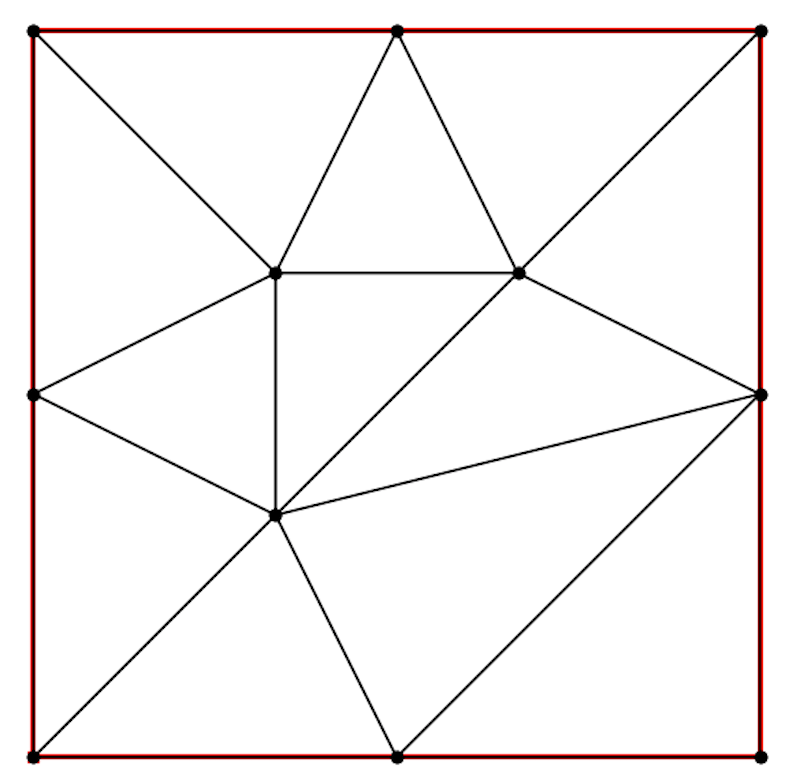
\includegraphics[width=0.45\textwidth]{images/ex1/mesh}}
		\caption{Контур и триангуляция квадратного пруда.}
	\end{figure}
\end{frame}

\begin{frame}
\frametitle{Квадратный пруд без островов}
	\begin{figure}[H]
		\centering
		\subfloat{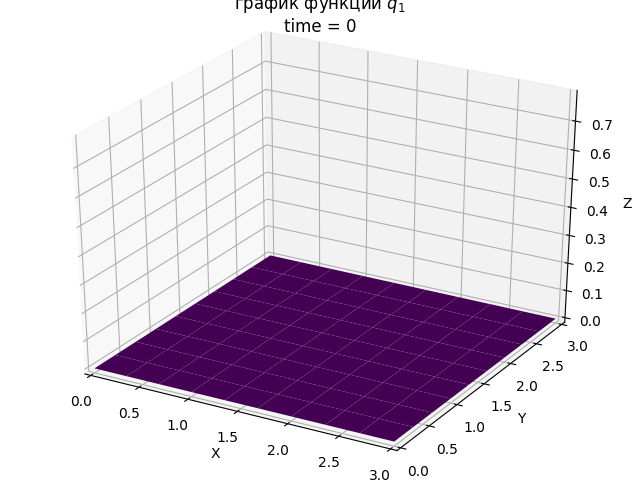
\includegraphics[width=0.41\textwidth]{images/ex1/q_1/0}}
		\hfill
		\subfloat{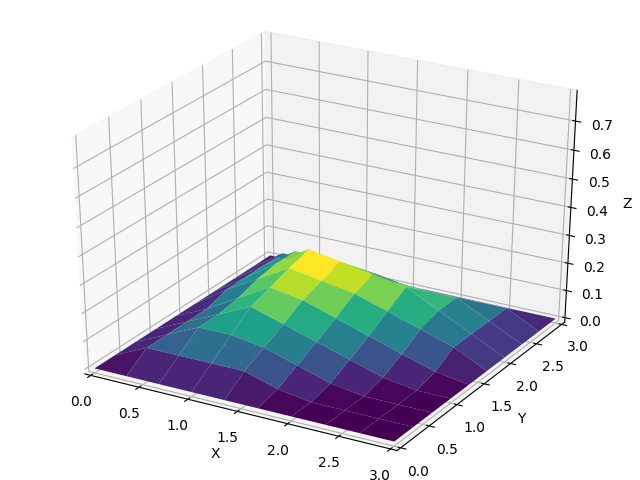
\includegraphics[width=0.41\textwidth]{images/ex1/q_1/1}}
		\hfill
		\subfloat{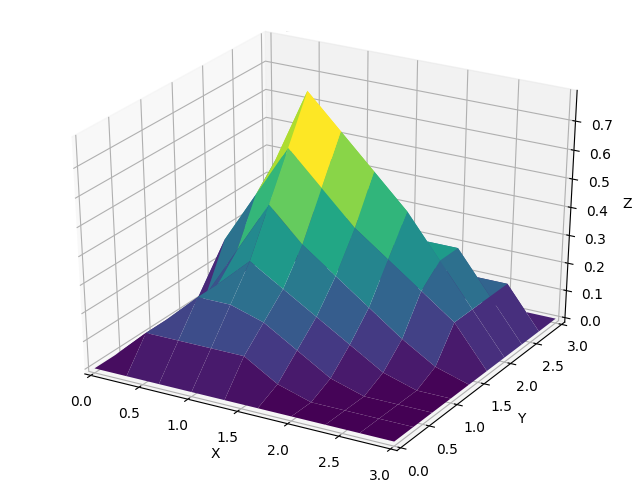
\includegraphics[width=0.41\textwidth]{images/ex1/q_1/2}}
		\caption{Изменение проекции потока жидкости на ось $x_1$.}
	\end{figure}
\end{frame}

\begin{frame}
\frametitle{Квадратный пруд без островов}
	\begin{figure}[H]
		\centering
		\subfloat{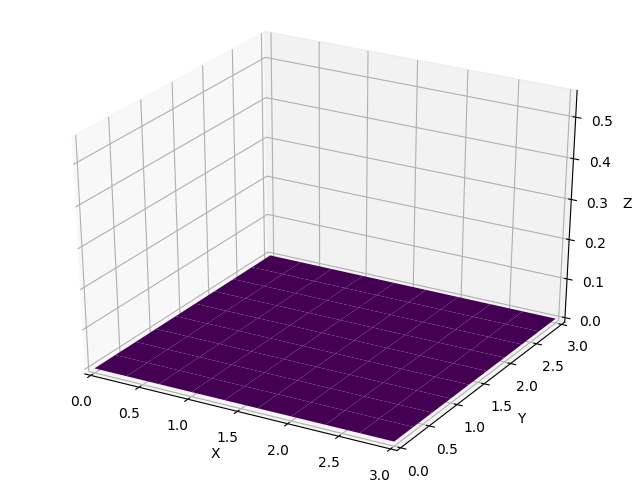
\includegraphics[width=0.41\textwidth]{images/ex1/q_2/0}}
		\hfill
		\subfloat{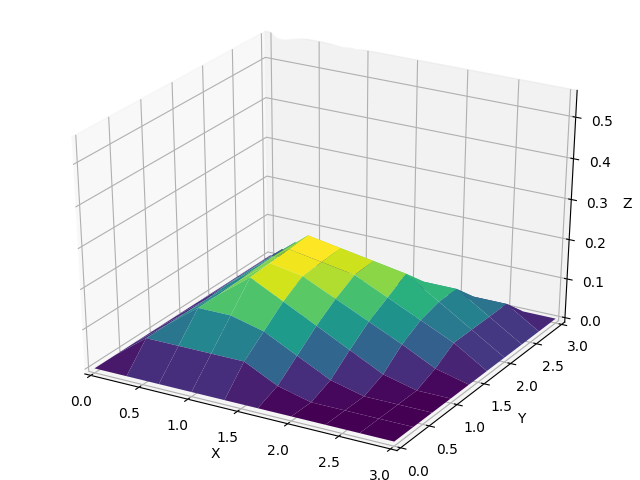
\includegraphics[width=0.41\textwidth]{images/ex1/q_2/1}}
		\hfill
		\subfloat{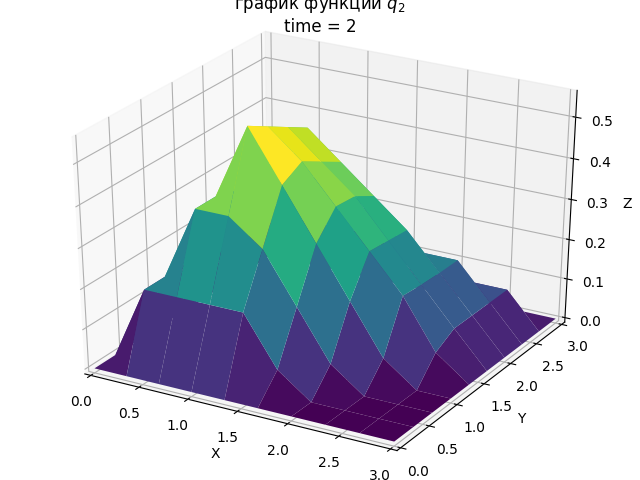
\includegraphics[width=0.41\textwidth]{images/ex1/q_2/2}}
		\caption{Изменение проекции потока жидкости на ось $x_2$.}
	\end{figure}
\end{frame}

\begin{frame}
\frametitle{Квадратный пруд без островов}
	\begin{figure}[H]
		\centering
		\subfloat{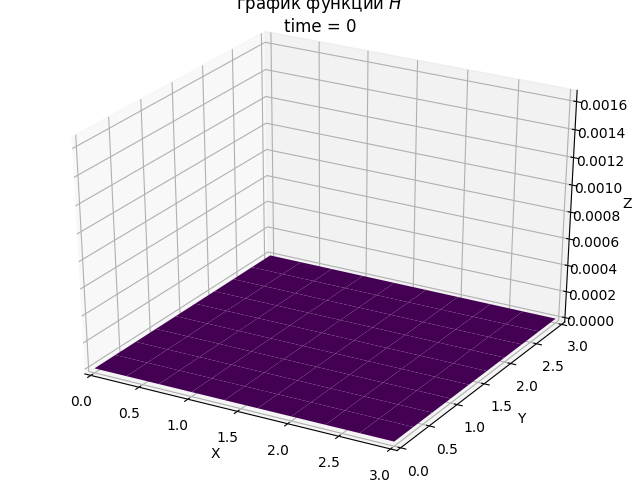
\includegraphics[width=0.41\textwidth]{images/ex1/H/0}}
		\hfill
		\subfloat{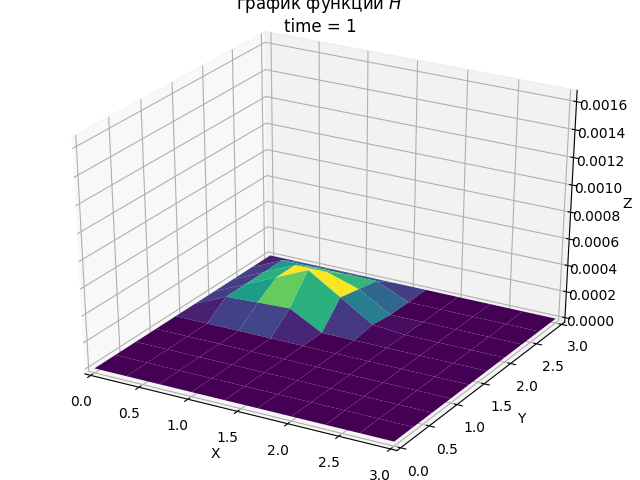
\includegraphics[width=0.41\textwidth]{images/ex1/H/1}}
		\hfill
		\subfloat{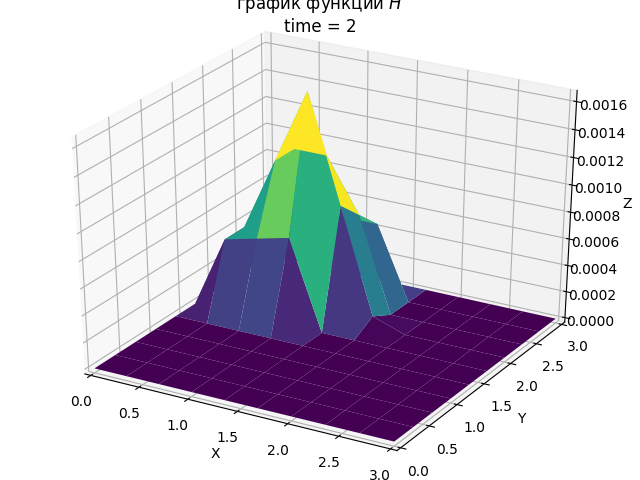
\includegraphics[width=0.41\textwidth]{images/ex1/H/2}}
		\caption{Изменение высоты.}
	\end{figure}
\end{frame}

\begin{frame}
\frametitle{Функция тока}
	\begin{equation}
		\Large\Psi = \int q_1(x_1, x_2) dx_2 = - \int q_2(x_1, x_2) dx_1
	\end{equation}
\end{frame}

\begin{frame}
\frametitle{Квадратный пруд без островов}
	\begin{figure}[H]
		\centering
		\subfloat{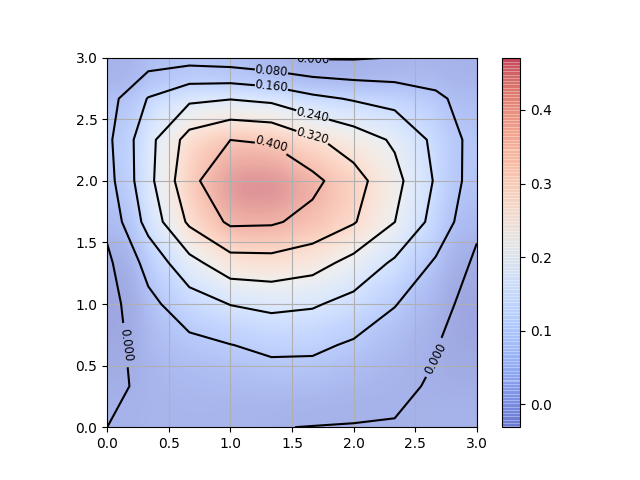
\includegraphics[width=0.49\textwidth]{images/ex1/psi/1}}
		\hfill
		\subfloat{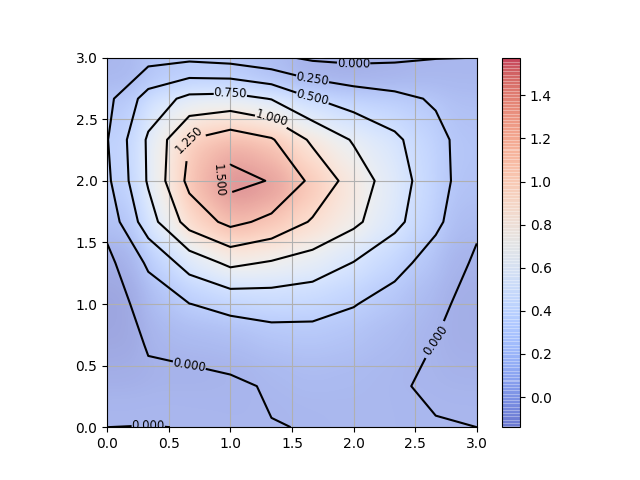
\includegraphics[width=0.49\textwidth]{images/ex1/psi/2}}
		\caption{Изменение функции тока.}
	\end{figure}
\end{frame}

\begin{frame}
\frametitle{Озеро Эльтон}
	\begin{figure}[H]
		\centering
		\subfloat{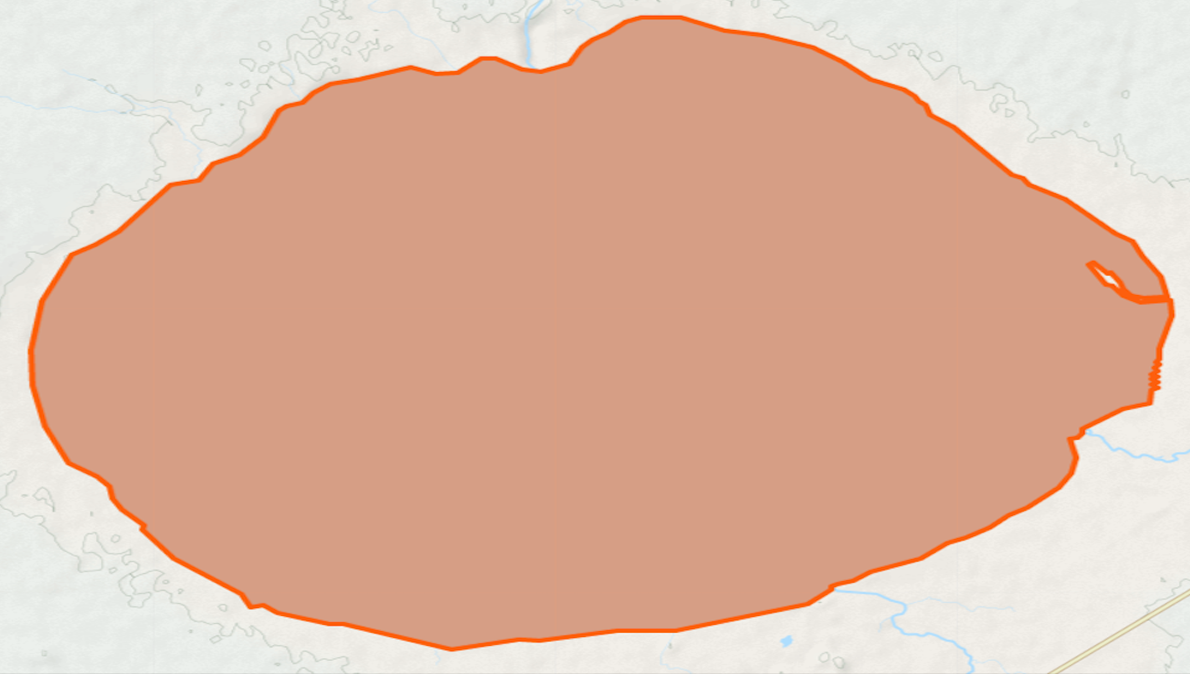
\includegraphics[width=0.49\textwidth]{images/slides/lake_elton}}
		\hfill
		\subfloat{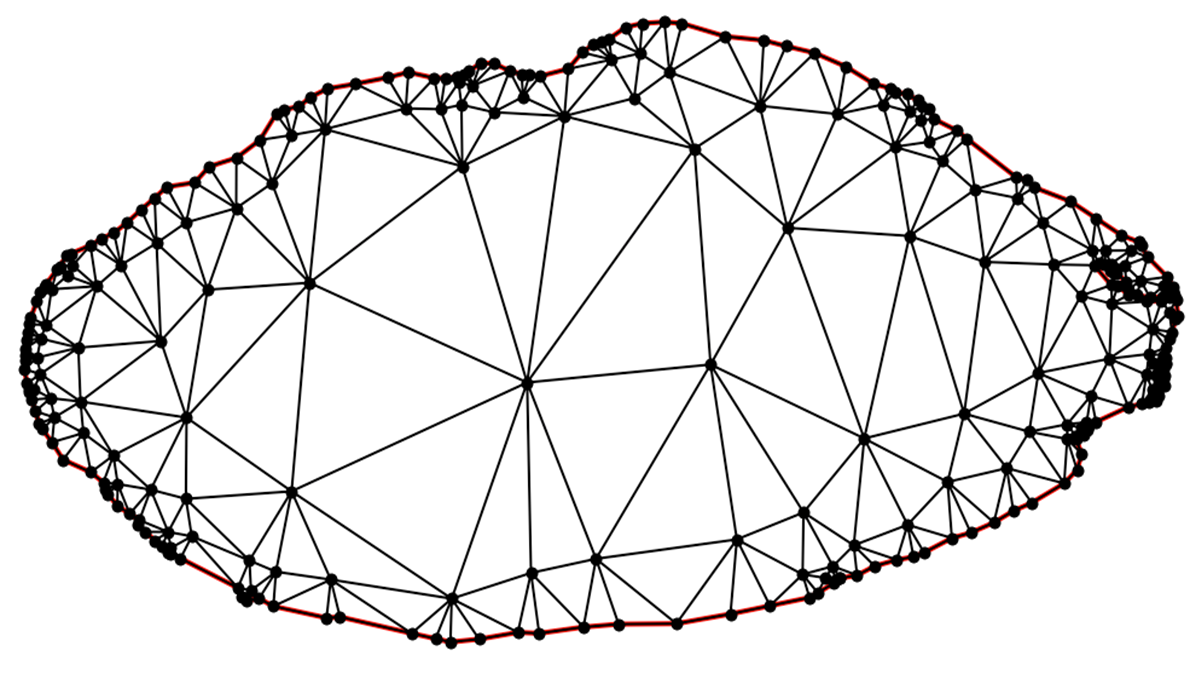
\includegraphics[width=0.49\textwidth]{images/slides/lake_elton_mesh}}
		\caption{Контур и триангуляция озера Эльтон.}
	\end{figure}
\end{frame}

\begin{frame}
\frametitle{Озеро Эльтон}
	\begin{figure}[H]
		\centering
		\subfloat{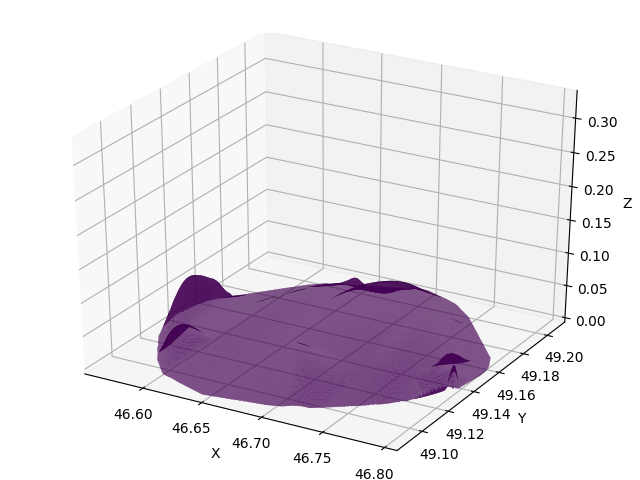
\includegraphics[width=0.49\textwidth]{images/ex2/q_1/902}}
		\hfill
		\subfloat{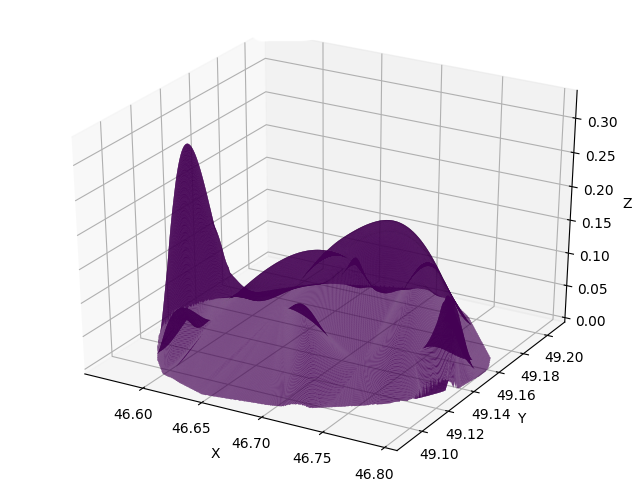
\includegraphics[width=0.49\textwidth]{images/ex2/q_1/905}}
		\caption{Изменение проекции потока жидкости на ось $x_1$.}
	\end{figure}
\end{frame}

\begin{frame}
\frametitle{Озеро Эльтон}
	\begin{figure}[H]
		\centering
		\subfloat{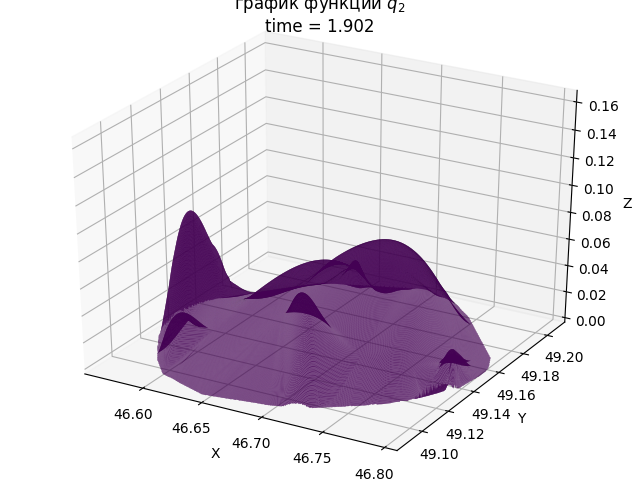
\includegraphics[width=0.49\textwidth]{images/ex2/q_2/902}}
		\hfill
		\subfloat{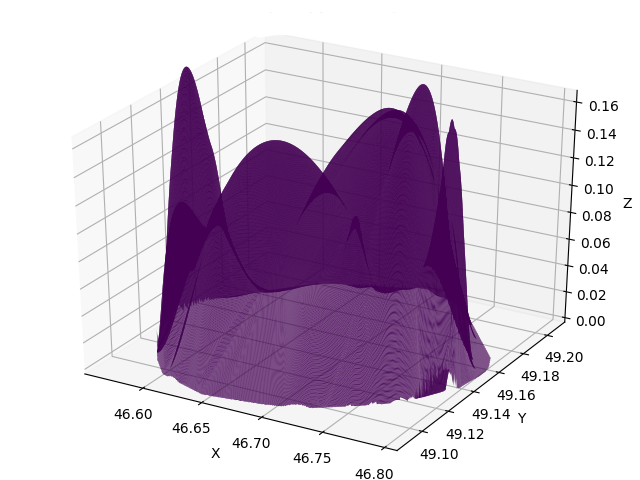
\includegraphics[width=0.49\textwidth]{images/ex2/q_2/905}}
		\caption{Изменение проекции потока жидкости на ось $x_2$.}
	\end{figure}
\end{frame}

\begin{frame}
\frametitle{Озеро Эльтон}
	\begin{figure}[H]
		\centering
		\subfloat{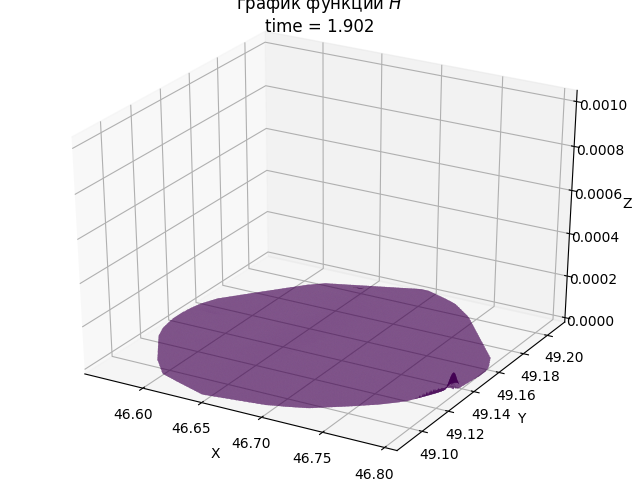
\includegraphics[width=0.49\textwidth]{images/ex2/H/902}}
		\hfill
		\subfloat{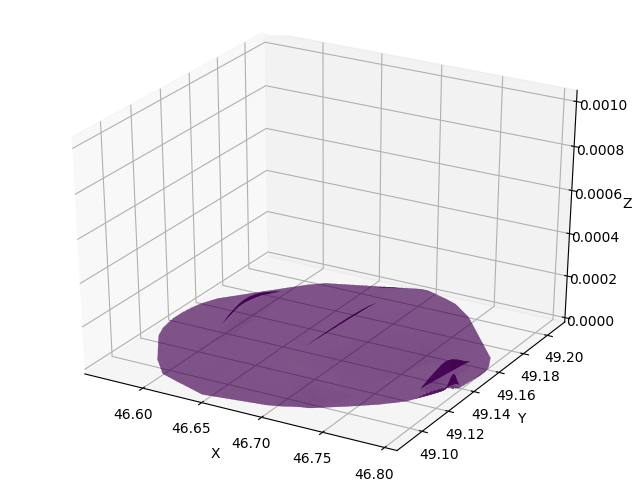
\includegraphics[width=0.49\textwidth]{images/ex2/H/905}}
		\caption{Изменение высоты в различные промежутки времени.}
	\end{figure}
\end{frame}

\begin{frame}
\frametitle{Озеро Эльтон}
	\begin{figure}[H]
		\centering
		\subfloat{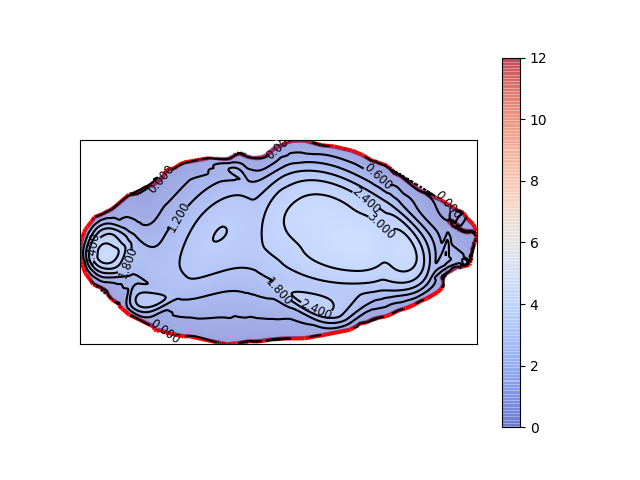
\includegraphics[width=0.49\textwidth]{images/ex2/psi/902}}
		\hfill
		\subfloat{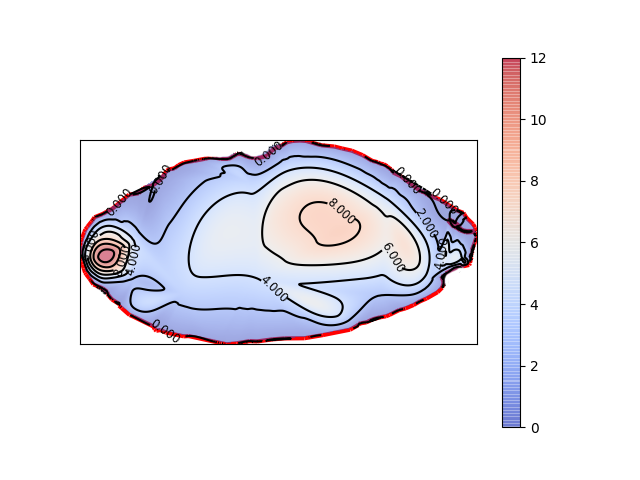
\includegraphics[width=0.49\textwidth]{images/ex2/psi/905}}
		\caption{Изменение функции тока в различные промежутки времени.}
	\end{figure}
\end{frame}

\begin{frame}
\frametitle{Квадратный пруд с островами}
	\begin{figure}[H]
		\centering
		\subfloat{
\includegraphics[width=0.45\textwidth]{images/ex3/contour}}
		\hfill
		\subfloat{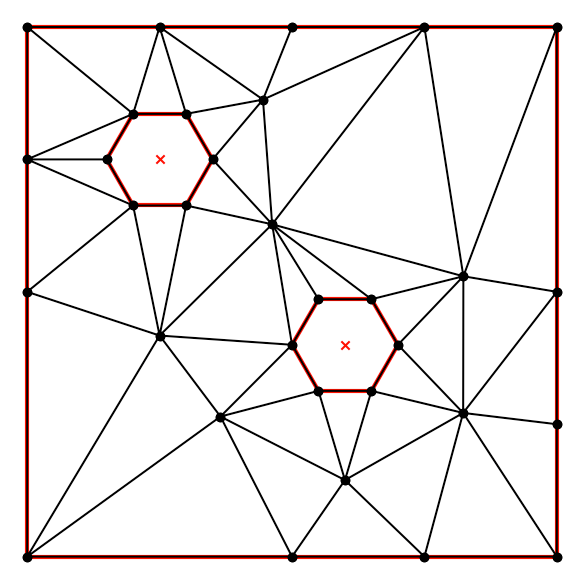
\includegraphics[width=0.45\textwidth]{images/ex3/mesh}}
		\caption{Контур и триангуляция квадратного пруда с островами.}
	\end{figure}
\end{frame}

\begin{frame}
\frametitle{Квадратный пруд с островами}
	\begin{figure}[H]
		\centering
		\subfloat{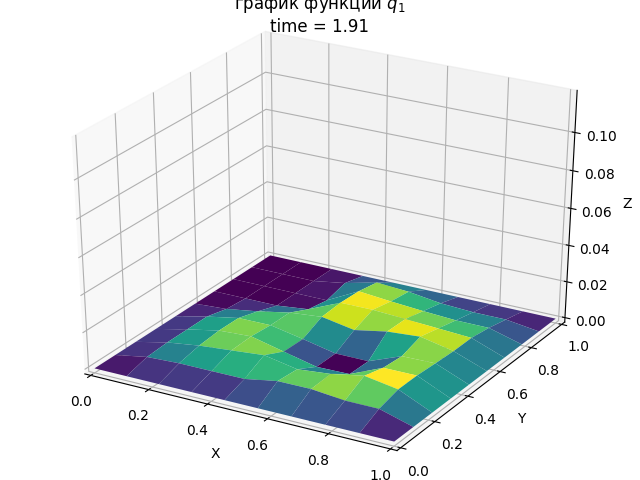
\includegraphics[width=0.49\textwidth]{images/ex3/q_1/91}}
		\hfill
		\subfloat{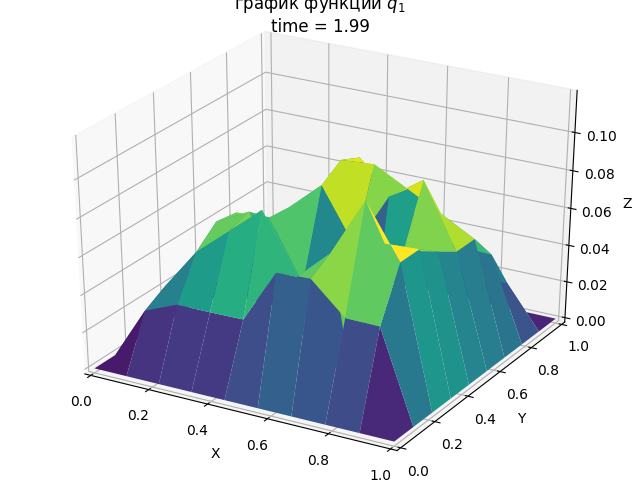
\includegraphics[width=0.49\textwidth]{images/ex3/q_1/99}}
		\caption{Изменение проекции потока жидкости на ось $x_1$.}
		\end{figure}
\end{frame}

\begin{frame}
\frametitle{Квадратный пруд с островами}
	\begin{figure}[H]
		\centering
		\subfloat{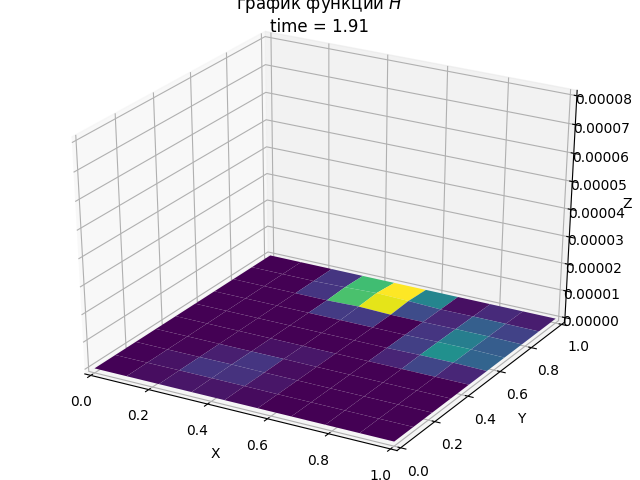
\includegraphics[width=0.49\textwidth]{images/ex3/H/91}}
		\hfill
		\subfloat{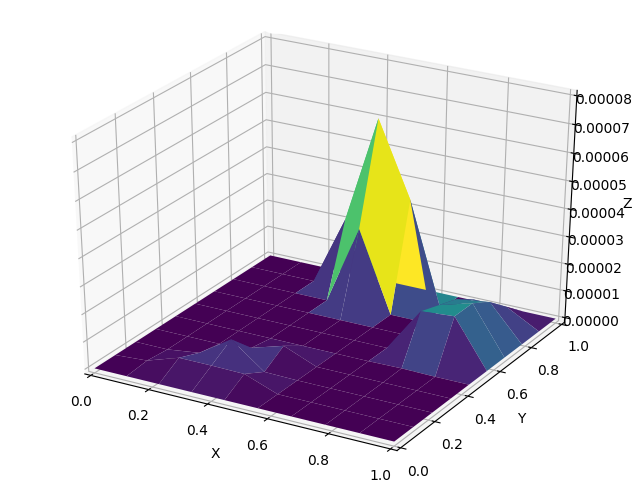
\includegraphics[width=0.49\textwidth]{images/ex3/H/99}}
		\caption{Изменение высоты в различные промежутки времени.}
	\end{figure}
\end{frame}

\begin{frame}
\frametitle{Квадратный пруд с островами}
	\begin{figure}[H]
		\centering
		\subfloat{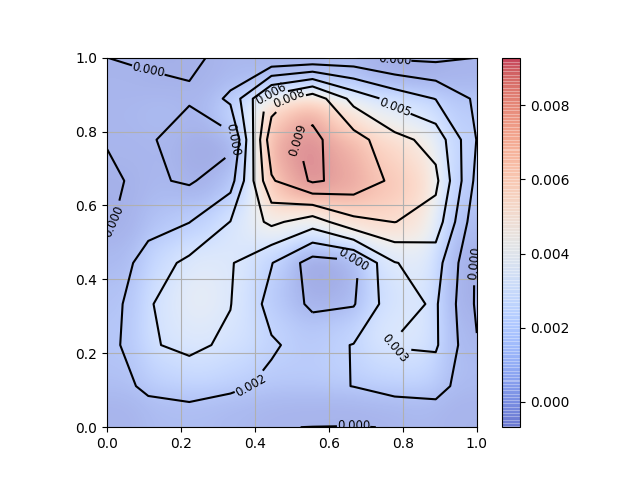
\includegraphics[width=0.49\textwidth]{images/ex3/psi/91}}
		\hfill
		\subfloat{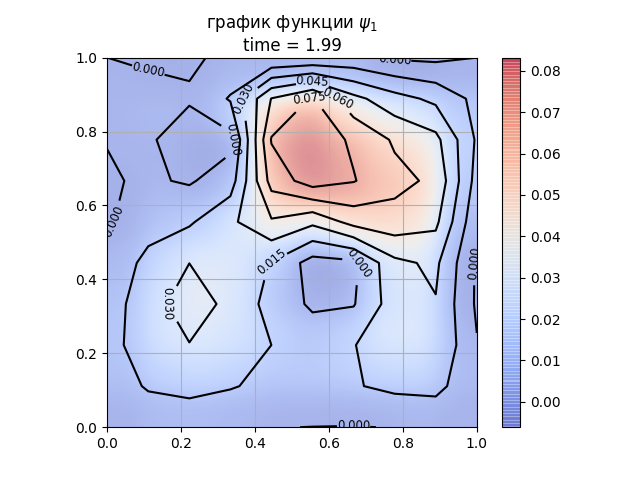
\includegraphics[width=0.49\textwidth]{images/ex3/psi/99}}
		\caption{Изменение функции тока.}
	\end{figure}
\end{frame}

\begin{frame}
\frametitle{Озеро Верхнее}
	\begin{figure}[H]
		\centering
		\subfloat{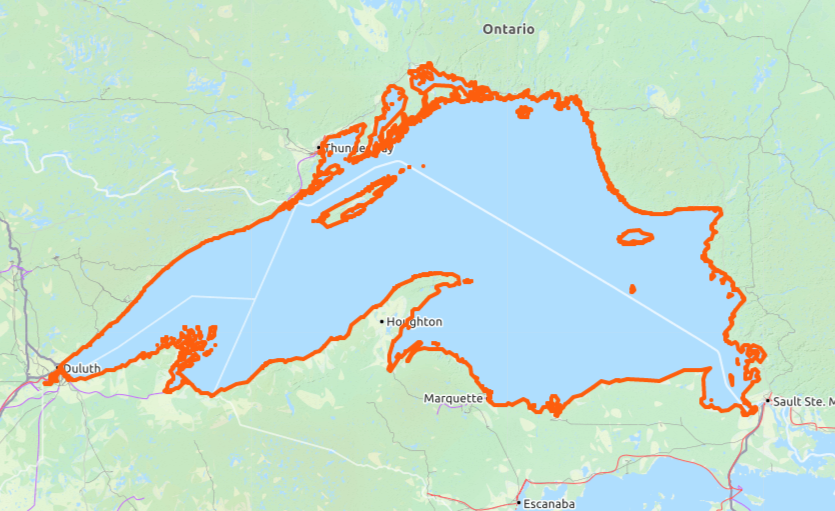
\includegraphics[width=0.49\textwidth]{images/ex4/lake_superior}}
		\hfill
		\subfloat{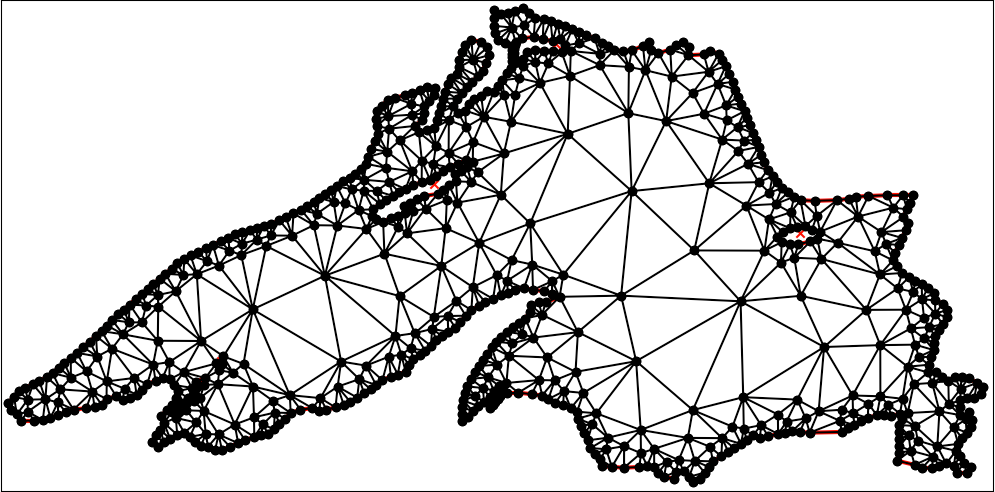
\includegraphics[width=0.49\textwidth]{images/ex4/mesh}}
		\caption{Контур и триангуляция озера Верхее.}
	\end{figure}
\end{frame}

\begin{frame}
\frametitle{Озеро Верхнее}
	\begin{figure}[H]
		\centering
		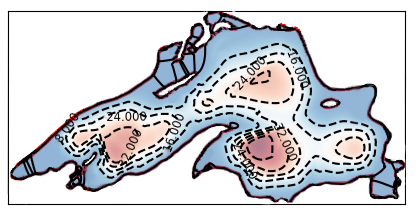
\includegraphics[width=0.9\linewidth]{images/ex4/psi/1}
		\caption{График функции тока.}
	\end{figure}
\end{frame}

\begin{frame}
\frametitle{БД для хранения результатов}
	\begin{figure}[H]
		\centering
		
\includegraphics[width=0.8\linewidth]{images/slides/logo/mongo}
	\end{figure}
\end{frame}

\begin{frame}
\frametitle{БД для хранения результатов}
	\begin{figure}[H]
		\centering
		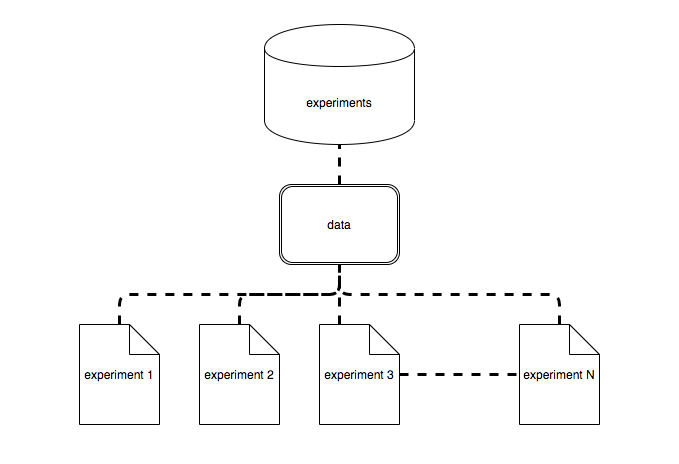
\includegraphics[width=1.0\linewidth]{images/database}
		\caption{Структура БД.}
	\end{figure}
\end{frame}

\begin{frame}[c]
\begin{center}
\frametitle{\LARGE Спасибо за внимание!}

{\LARGE \inserttitle}

\bigskip

{\insertauthor} 

\bigskip\bigskip

{\insertinstitute}

\bigskip\bigskip

{\large \insertdate}
\end{center}
\end{frame}

\end{document}